\newgeometry{top=1cm, bottom=2cm}
\section{Lineare Gleichungssysteme}
\begin{figure}[h!]
    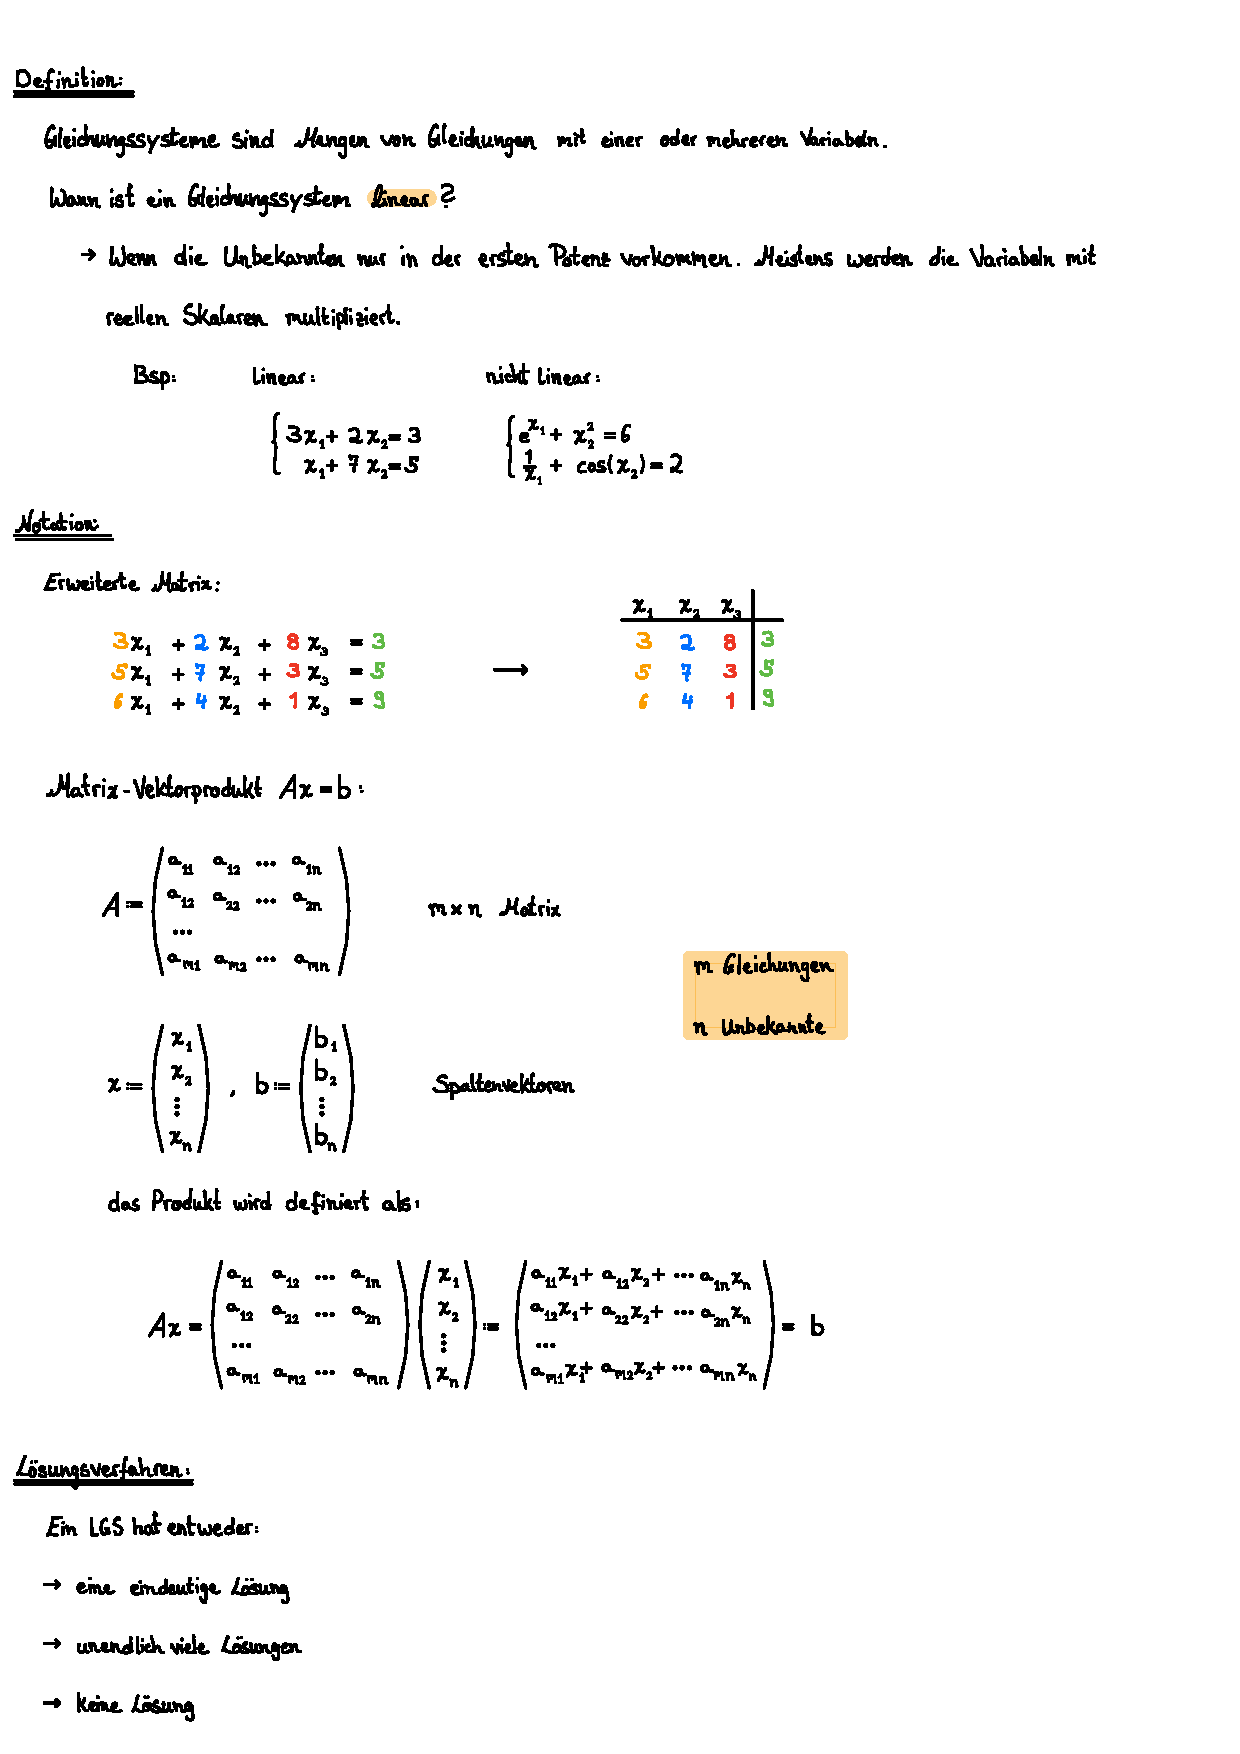
\includegraphics[page=1, scale=0.842]{pdf/01_Lineare_Gleichungssysteme.pdf}
\end{figure}
\newpage
\includepdf[pages={2-}, 
            pagecommand={\thispagestyle{plain}}, 
            scale=0.95]{pdf/01_Lineare_Gleichungssysteme.pdf}
            
\newgeometry{top=2.5cm, bottom=2cm}
\subsection{Beispielaufgaben}
\vspace{1cm}

\subsubsection{}  %Buch Seite 18 keine Lösungen
Für welche Werte des Parameters \( a \) hat das Gleichungssystem

\begin{equation*}
    \begin{aligned}
        a&x_1 +& 4&x_2 &+ 5x_3 &= a\\
        1&x_1 +& a&x_2 &- 2x_3 &= 1\\
        2&x_1 +& 2a&x_2 &- a^2x_3 &= a
    \end{aligned}   
\end{equation*}

keine, genau eine oder unendlich viele Lösungen? Bestimmen Sie jeweils auch die Lösungsmenge.

\vspace{1\baselineskip}

\begin{solution}

    \vspace{1\baselineskip}

    Schreibe hier die Lösung

\end{solution}

\newpage

\subsubsection{} %Buch Seite 18 keine Lösungen
Geben Sie für \( a \) und \( b \) Bedingungen an, so dass das System
\begin{equation*}
    \begin{aligned}
        0 &x_1 &+ a &x_2 &+ 1 &x_3 &= -b\\
        a &x_1 &+ 0 &x_2 &+ b &x_3 &= -1\\
        a &x_1 &+ a &x_2 &+ 2 &x_3 &= -2
    \end{aligned}
\end{equation*}

\begin{enumerate}[label=\alph*)]
    \item eine Lösungsmenge mit \textit{zwei} freien Parametern besitzt.
    \item eine Lösungsmenge mit \textit{einem} freien Parameter besitzt.
    \item eindeutig lösbar ist.
    \item keine Lösung hat.
\end{enumerate}

Geben Sie sie für alle Fälle a), b), c) die Lösungsmenge an.\\

\noindent \textbf{Lösung:}